\documentclass{article}

\usepackage{repsty}

\newcommand{\nb}{{n_b}}

\newcommand{\uvec}[1]{\boldsymbol{\hat{#1}}}
\newcommand{\abs}[1]{\vert#1\vert}
\newcommand{\proj}[2]{\pi_{\uvec{#2}}\vec{#1}}

\newcommand{\deq}{\overset{\Delta}{=}}

\newcommand{\Norm}{\mathcal{N}}

\begin{document}

\section*{Introduction}
In this note we try to derive the form of the measured signal, as well as investigate its properties under the assumption of a finite particle phase and oscillation frequency distributions.

\section{Projection of polarization}
The polarization of the beam is the sum of the spins of the particles in it. We measure the projection of the polarization on the $y$-axis:
\begin{align}
	\vec{P} &= \sum_{i=1}^\nb \vec{s}, \notag\\
	\proj{s}{y} &\equiv \uvec{y}\cdot\vec{s} = \abs{\vec{s}}\cos\Theta, \notag\\
	\proj{P}{y}(t) &= \sum_i \proj{s_i}{y} = \abs{\vec{s}}\sum_i \cos\Theta_i(t), \label{eq:SumSpins}\\
	\Theta_i(t) &= \omega_i\cdot t + \phi_i.\notag
\end{align}

The signal at time $t$ is a sum of random variables, and hence has expectation 
\begin{align*}
	\Xpct{\proj{P}{y}(t)} &= \abs{\vec{s}}\sum_i\Xpct{\cos\Theta_i(t)} = \abs{\vec{s}}\sum_i\int_{\infty}\cos x \cdot f_{\Theta_i(t)}(x)\td x \\
	&= \abs{\vec{s}}\sum_i\int_{-1}^{+1} f_{\Theta_i(t)}(\arcsin y)\td y.
\end{align*}

\subsection{Distribution of $\Theta_i(t)$}
\newcommand{\f}[1]{f_{#1}}
\newcommand{\fw}{\f{\omega}}
\newcommand{\fp}{\f{\phi}}
\newcommand{\fwt}{\f{\omega t}}
\newcommand{\ftht}{\f{\Theta(t)}}

\newcommand{\wycoef}{G}
\newcommand{\dy}{\Delta\gamma}

If the distribution of $\omega_i$ is $\fw(x)$, then that of $\omega_i t$ is $\fwt(x) = \frac{1}{t}\fw(\frac{x}{t})$. The distribution of $\Theta_i(t)$ is the convolution 
\[
	(\fwt*\fp)(\theta) \deq \int_\infty \fwt(\theta-y)\fp(y)\td y = \frac1t \int_\infty \fw\bkt{\frac{\theta-y}{t}}\fp(y)\td y.
\]

Assuming $\omega_i = \omega_0 + \wycoef\dy_i^2$ and $f_{\dy}(y)=\Norm(0, \SD{\dy})(y)$, 
\begin{equation*}
	\f{\dy^2}(y) =\begin{cases}
		\frac1{\SD{\dy}^2} \cdot\chi^2_1(\frac{y}{\SD{\dy}^2}), & y \geq 0,\\
		0, & y < 0;
	\end{cases}
\end{equation*}
and
\begin{equation}\label{eq:DistW}
	\fw(x) =\begin{cases}
		 \frac{1}{\wycoef\SD{\dy}^2}\chi_1^2\bkt{\frac{x-\omega_0}{\wycoef\SD{\dy}^2}}, & x\geq \omega_0,\\
		 0 & x < \omega_0.
	\end{cases}
\end{equation} 

\DeclareDocumentCommand{\A}{s}{\IfBooleanTF{#1}{\frac{a\exp(\frac12 a\omega_0)}{\sqrt{2\pi a}}}{A(a,\omega_0)}}
\begin{equation*}
	\fw(x) = \begin{cases}
		\A\cdot \frac{\exp(-\frac12 a x)}{\sqrt{x-\omega_0}}, & x \geq \omega_0, \\
		0, & x < \omega_0,
	\end{cases}
\end{equation*}
with
\begin{equation}
	\A \equiv \A*, ~~ a \equiv \frac{1}{G\SD{\dy}^2}.
\end{equation}

\DeclareDocumentCommand{\B}{s}{\IfBooleanTF{#1}{\sqrt{t}\exp\bkt{ -\frac{a\theta}{2t} } }{B(\theta, t)}}
\DeclareDocumentCommand{\agl}{s}{\IfBooleanTF{#1}{\theta-\omega_0t}{\Delta\theta(t)}}
\begin{equation*}
	\fw\bkt{\frac{\theta-y}{t}} = \begin{cases}
		\A\cdot\B\cdot\frac{\exp\bkt{\frac{ay}{2t}}}{\sqrt{\agl-y}}, & y \leq \agl,\\
		0, & y > \agl,
	\end{cases}
\end{equation*}
where 
\begin{equation}
	\B \equiv \B*, ~~ \agl \equiv \agl*.
\end{equation}

We'll assume a normally distributed $\phi_i\sim\Norm(\phi_0, \SD{\phi})$.

\newcommand{\sdp}{\SD{\phi}}
\DeclareDocumentCommand{\C}{s}{
		\IfBooleanTF{#1}{ \exp\bkt{\frac{\phi_0^2}{\sdp^2}} }{ C(\phi_0,\sdp) }
}
\DeclareDocumentCommand{\X}{s}{\IfBooleanTF{#1}{\frac{a\sdp^2 + 4t\phi_0}{2t\sdp^2}}{\xi}}
\DeclareDocumentCommand{\CDF}{s}{\IfBooleanTF{#1}{\int_{-\infty}^{\agl}\frac{\exp(\X y - \sfrac{y^2}{\sdp^2})}{\sqrt{\agl - y}}\td y}{D(\theta, \omega_0t)}}

Hence, 
\begin{align*}
	\ftht(\theta) = (\fwt*\fp)(\theta) = \frac1t\A\C\cdot\B\CDF,
\end{align*}
where 
\begin{align}
		\CDF \equiv \CDF*, \\ \C \equiv \C*, ~~ \X \equiv \X*.
\end{align}

\section{Simulation}
\newcommand{\ytcoef}{h}
\newcommand{\dwcoef}{g}
\newcommand{\vp}[2]{{#1}\cdot 10^{#2} }

\subsection{$\wycoef$}
From eq.~\eqref{eq:DistW}, $\var{\frac{\omega}{\wycoef\SD{\dy}^2}} = \bkt{\wycoef\SD{\dy}^2}^{-2}\cdot\var{\omega}  = 2$, hence $\var{\omega} = 2\bkt{\wycoef\SD{\dy}^2}^2$.

$\var{\omega T} = T^2\cdot \var{\omega} = 2T^2\bkt{\wycoef\SD{\dy}^2}^2$; $\SD{\omega T} = \sqrt{2}\cdot T\cdot \wycoef\SD{\dy}^2$.

Therefore, for $\wycoef$ we have
\begin{equation}
	\wycoef = \frac{\SD{\omega T}}{\sqrt{2}\cdot T\cdot \SD{\dy}^2}.
\end{equation}

If in $T=1000$ secs $\SD{\omega T} = 1$ rad, assuming $\SD{\dy} = \vp{1}{-3}$, $\wycoef \approx \vp{7}{2}$.

In the simulation, the following model was assumed:\\
\begin{minipage}{.5\textwidth}
	\begin{align*}
		\dy &\sim \Norm(0, \SD{\dy}), \\
		\SD{\dy}(t) &= \SD{\dy}(0) + \ytcoef\cdot t, \\
		\omega_i &= \omega_0 + \wycoef\cdot \dy_i^2, \\
		\phi_i &\sim \Norm(\phi_0, \SD{\phi}).
	\end{align*}
\end{minipage}
\begin{minipage}{.5\textwidth}
	\begin{tabular}{clr}
		  Parameter   & Value            &          Dimension \\ \hline
		$\SD{\dy}(0)$ & $\vp{1}{-3}$     &  \\
		  $\ytcoef$    & $\vp{5}{-6}$     &   $\sfrac{1}{sec}$ \\
		 $\omega_0$   & $3$              & $\sfrac{rad}{sec}$ \\
		  $\wycoef$    & $\vp{7}{2}$      & $\sfrac{rad}{sec}$ \\
		  $\phi_0$    & $\sfrac{\pi}{2}$ &  \\
		 $\SD{\phi}$  & $\vp{2}{-2}$     &              $rad$ \\ \hline
	\end{tabular}
\end{minipage}


\subsection{Constant $\SD{\dy}(t=0)$}
In order to have unchanging distributions of the beam particles' phase and oscillation frequency presented in Figure~\ref{fig:PSdist_cDy} we sampled $\omega_i,~\phi_i$ once at $t=0$, and only changed the time variable in eq.~\eqref{eq:SumSpins}. The resulting polarization signal has the form shown in Figure~\ref{fig:Sgl_cDyPhys}.
\begin{figure}[h]
	\begin{subfigure}[b]{.45\textwidth}
		\centering
		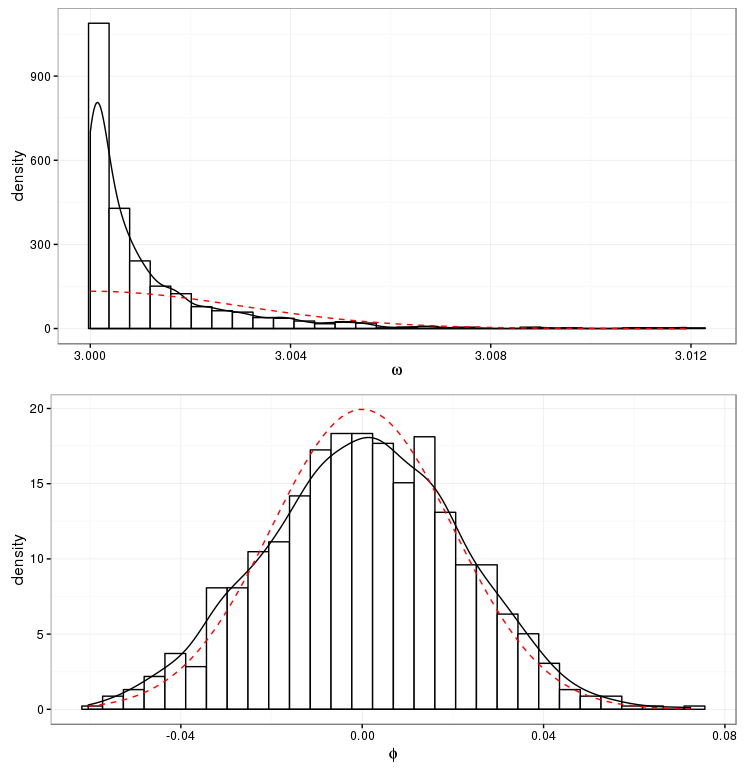
\includegraphics[scale=.5]{../img/PS_dist}
		\caption{Phase space distributions.\label{fig:PSdist_cDy}}
	\end{subfigure}~~~~~~~~
	\begin{subfigure}[b]{.45\textwidth}
		\centering
		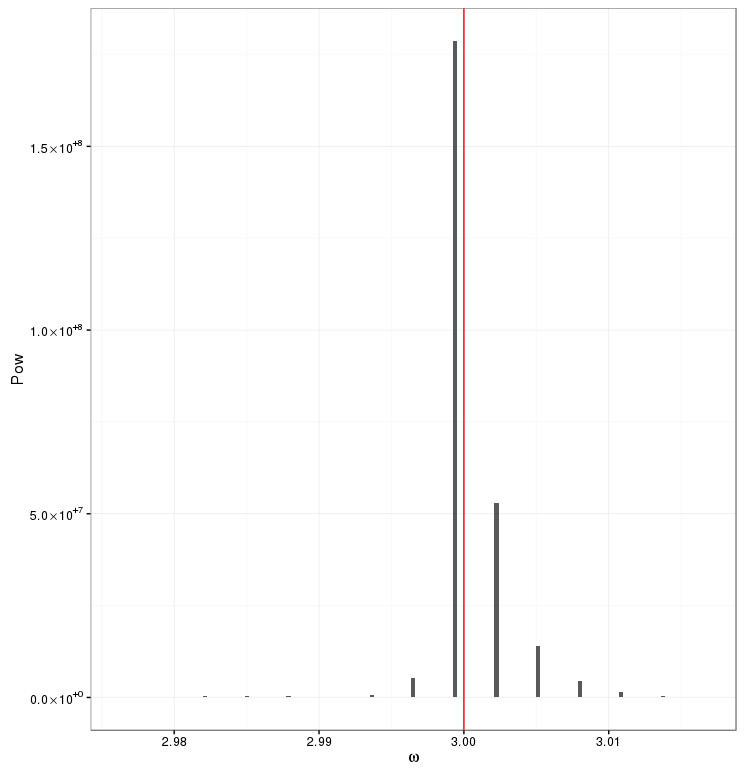
\includegraphics[scale=.5]{../img/Spec_PhysDistros}
		\caption{Power spectral density plot.\label{fig:PSD_cDyPhys}}
	\end{subfigure}
	\caption{Distributions and power spectra.}
\end{figure}
\begin{figure}[h]
	\centering
	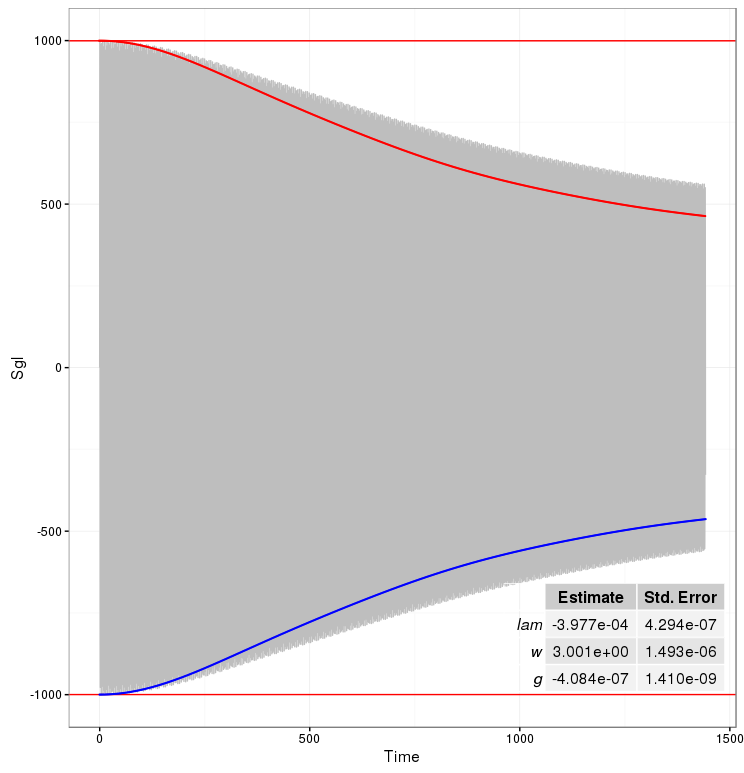
\includegraphics[scale=.6]{../img/Sgl_PhysDistros}
	\caption{Polarization signal in the case of constant phase space distributions. The black lines mark the measurements taken at the points $\sin(\omega_0\cdot t_n + \phi_0)=\pm 1$.\label{fig:Sgl_cDyPhys}}
\end{figure}

One can observe (the detailization in Figure~\ref{fig:Sgl_cDyPhys}) that the black lines, marking the measurements supposed to be at the peaks/valleys of the signal (the null envelope), fall in front of the actual extrema after a while, which suggests that the signal's oscillation frequency is greater than that of the synchronous particle, $\omega_0$. With that in mind, we fitted the function $f(t) = n_b\cdot\exp\bkt{\lambda t}\cdot\sin\bkt{(\omega+\dwcoef\cdot t)\cdot t + \phi_0}$ to the simulated data.

The model fit yielded an $\hat{\omega} \approx 3.001 \pm 1.535\cdot10^{-6}$, and a life-time $\hat{\tau}\approx 2600$ sec. The frequency growth factor, $g$, is estimated $\dwcoef < 0$, indicating a \emph{decreasing} oscillation frequency. The estimate of $g$ is statistically significant, with the t-value $\approx -270$; we note, however, that the used model is drastically misspecified,~\footnote{The first derivative of the signal's envelope falls much slower at the beginning.} which might be the cause of the contradiction between the supposed deceleration of oscillation, and the evidence of the computed envelope points. 

The signal's power spectrum (Figure~\ref{fig:PSD_cDyPhys}) mimics the particles' $\omega$ density distribution.

\subsection{Growing $\SD{\dy}(t)$}
In this simulation(Figure~), we resampled the $(\omega,\phi)$ phase space at each measurement time. The effect of the growth of $\SD{\dy}$ can be observed not only in that the signal decays much more rapidly ($\hat{\tau}\approx 454$ sec), but also in the increase of $\Xpct{\hat{\omega}}$ from $3.001$ to $3.002$, caused by the appearance of a greater number of particles with higher frequencies.
\begin{figure}[h]
	\centering
	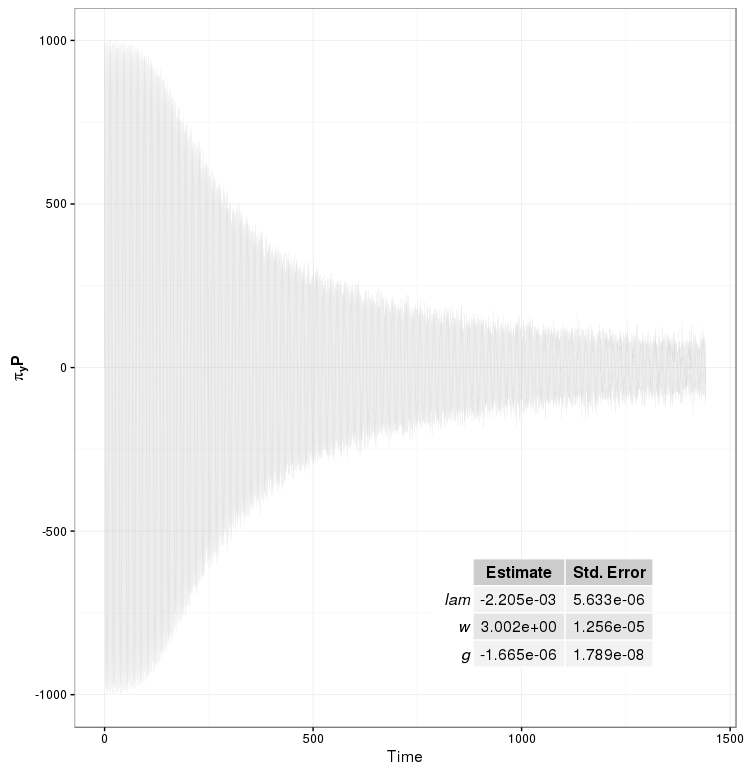
\includegraphics[scale=.6]{../img/Signal_Growing_Dgamma}
	\caption{Decoherence when $\SD{\dy}$ grows with time.}
\end{figure}

\subsection{Normally distributed $\omega$}
The $\fw,\fp$ distributions were kept constant throughout the simulation. In this case (Figure~\ref{fig:Sgl_cDyNorm}) the shift in the signal peaks from the null envelope is unnoticeable (as further evidenced by the non-convergence of the model with a frequency growth factor). Any systematic deviation of $\Xpct{\hat{\omega}}$ is due to the asymmetry of the $\omega$ distribution, and therefore decreases with the number of particles used in modeling.
\begin{figure}[h]
	\begin{subfigure}{.5\textwidth}
		\centering
		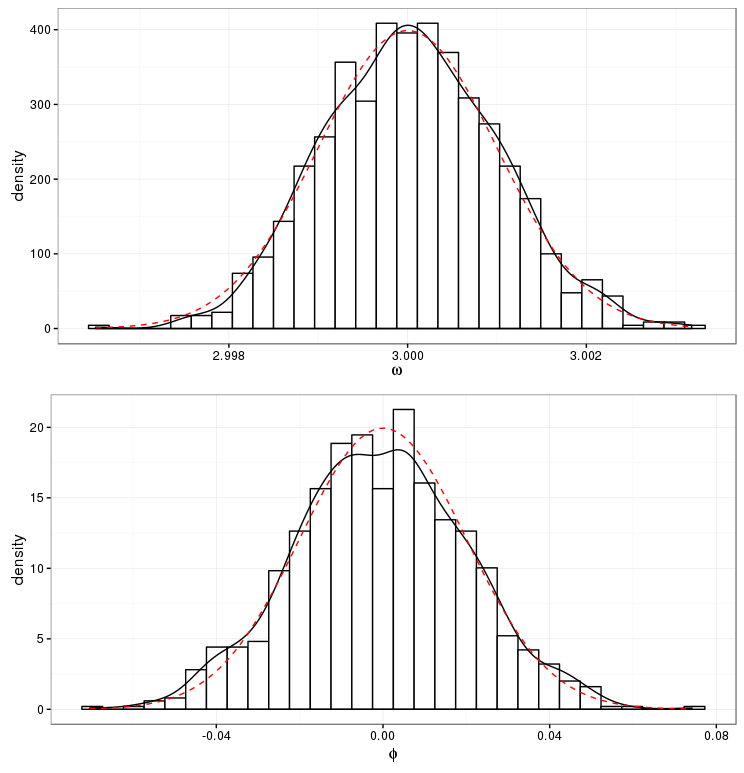
\includegraphics[scale=.5]{../img/PS_dist_Norm}
		\caption{Phase space distributions.}
	\end{subfigure}~
	\begin{subfigure}{.5\textwidth}
		\centering
		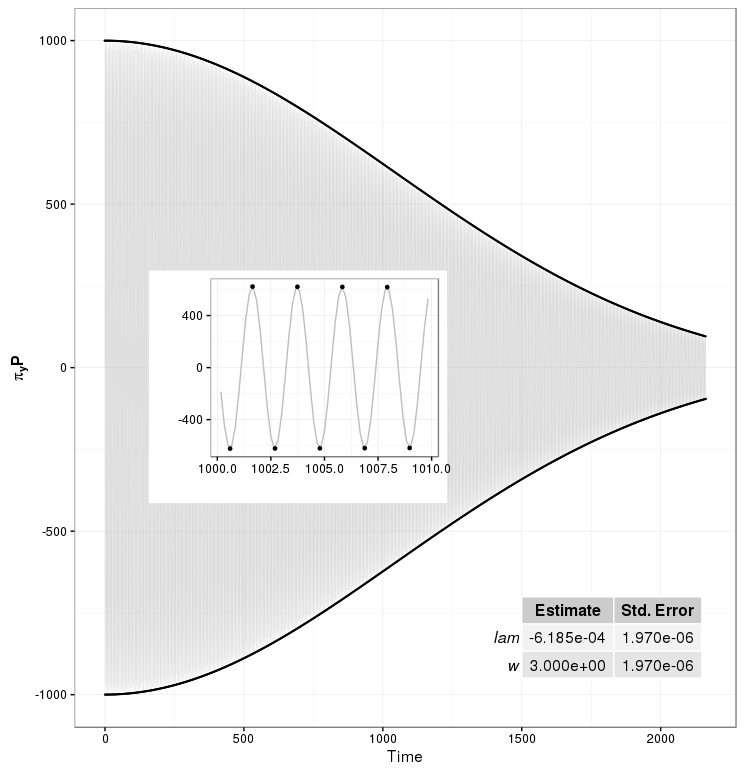
\includegraphics[scale=.5]{../img/Sgl_NormDistros}
		\caption{Signal in the case of a normally distributed oscillation frequency.}
	\end{subfigure}
	\caption{Normally distributed phase space variables.\label{fig:Sgl_cDyNorm}}
\end{figure}

\section{Envelope}


\end{document}